\section{Image Classification}

\subsection{Data-Driven Approach}

不同于传统的算法，统计机器学习的算法是\textbf{数据驱动}的。以图像分类任务为例，数据驱动方法包含以下 3 个步骤：

\begin{enumerate}
    \item 收集数据并标注；
    \item 使用机器学习方法训练一个分类器；
    \item 使用该分类器对新的图片进行分类。
\end{enumerate}

实现上，一个统计机器学习算法至少包含两个函数：\texttt{train} 和 \texttt{predict}，前者进行模型训练，后者使用训练好的模型进行预测。


\subsection{Nearest Neighbor}

最近邻分类器是最简单的分类器。仍然以图像分类为例，最近邻的 \texttt{train} 过程仅仅是记录下所有数据及其标签，\texttt{predict} 过程是选取数据集中与当前图片最相近的图片，并以其标签作为结果输出。

尽管最近邻很简单，但是仍然有一个问题需要解决：怎么评判两张图片的相似程度。由于图片可以看作像素点组成的 $H\times W\times C$ 向量，所以问题转化为两个向量相似程度的评判。设 $I_1,I_2$ 是要比较的两个图片向量，上标 $p$ 表示向量的第 $p$ 个元素，常用的距离有：

\begin{itemize}
    \item L1 distance（曼哈顿距离）：$d_1(I_1,I_2)=\sum_p|I_1^p-I_2^p|$
    \item L2 distance（欧几里得距离）：$d_2(I_1,I_2)=\sqrt{\sum_p(I_1^p-I_2^p)^2}$
\end{itemize}

最近邻分类器准确率较差，这是因为如果出现一个噪声点，它将对周围一圈产生误导，如下图所示。

\begin{figure}[H]
    \centering
    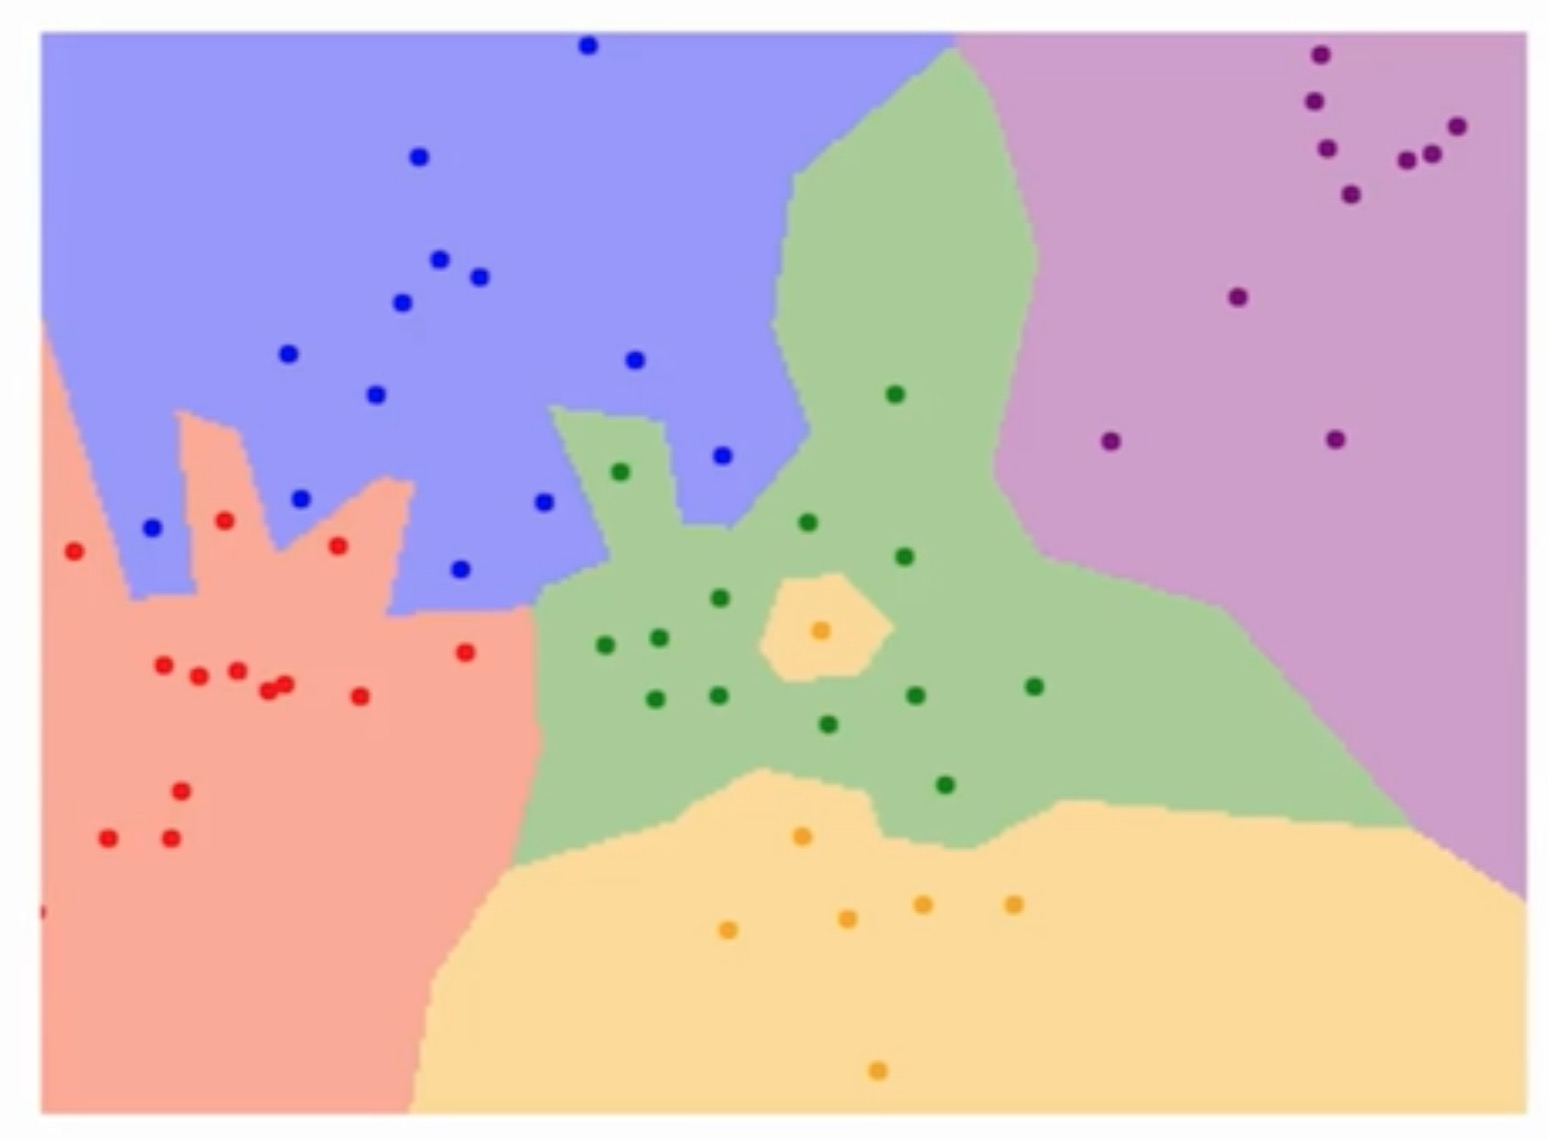
\includegraphics[width=0.3\linewidth]{figs/chapter1/nn.jpg}
\end{figure}

\subsection{K-Nearest Neighbor}

为了解决最近邻的问题，$k$ 近邻查看 $k$ 个最近的点，并以其中最多的标签作为结果。

\paragraph{超参数}

在 $k$ 近邻算法中，$k$ 如何取值是我们设定的，而非模型学习出的，这类参数被称作超参数。
$k$ 近邻算法的另一个超参数是距离函数的选取，选 $\text{L1 distance}$ 和选 $\text{L2 distance}$ 的结果会不同。

\begin{figure}[H]
    \centering
    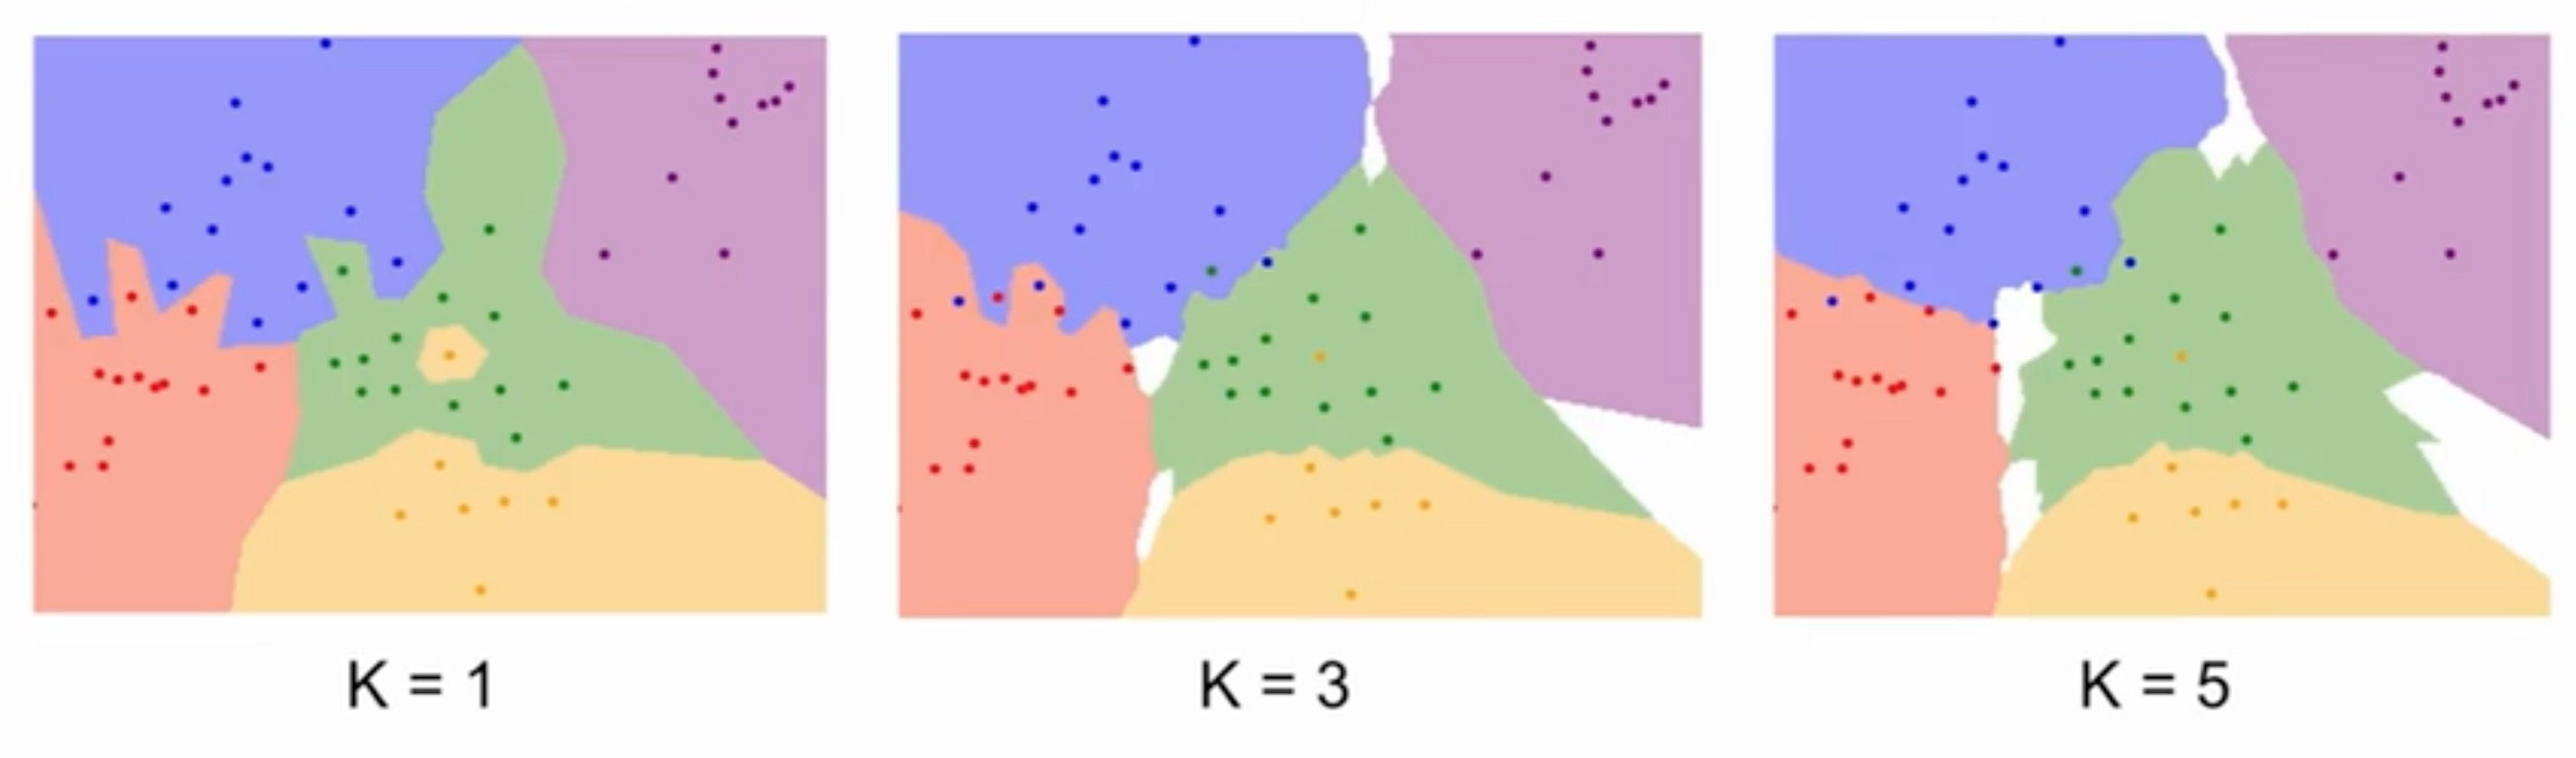
\includegraphics[width=0.8\linewidth]{figs/chapter1/knn k.jpg}
\end{figure}

\begin{figure}[H]
    \centering
    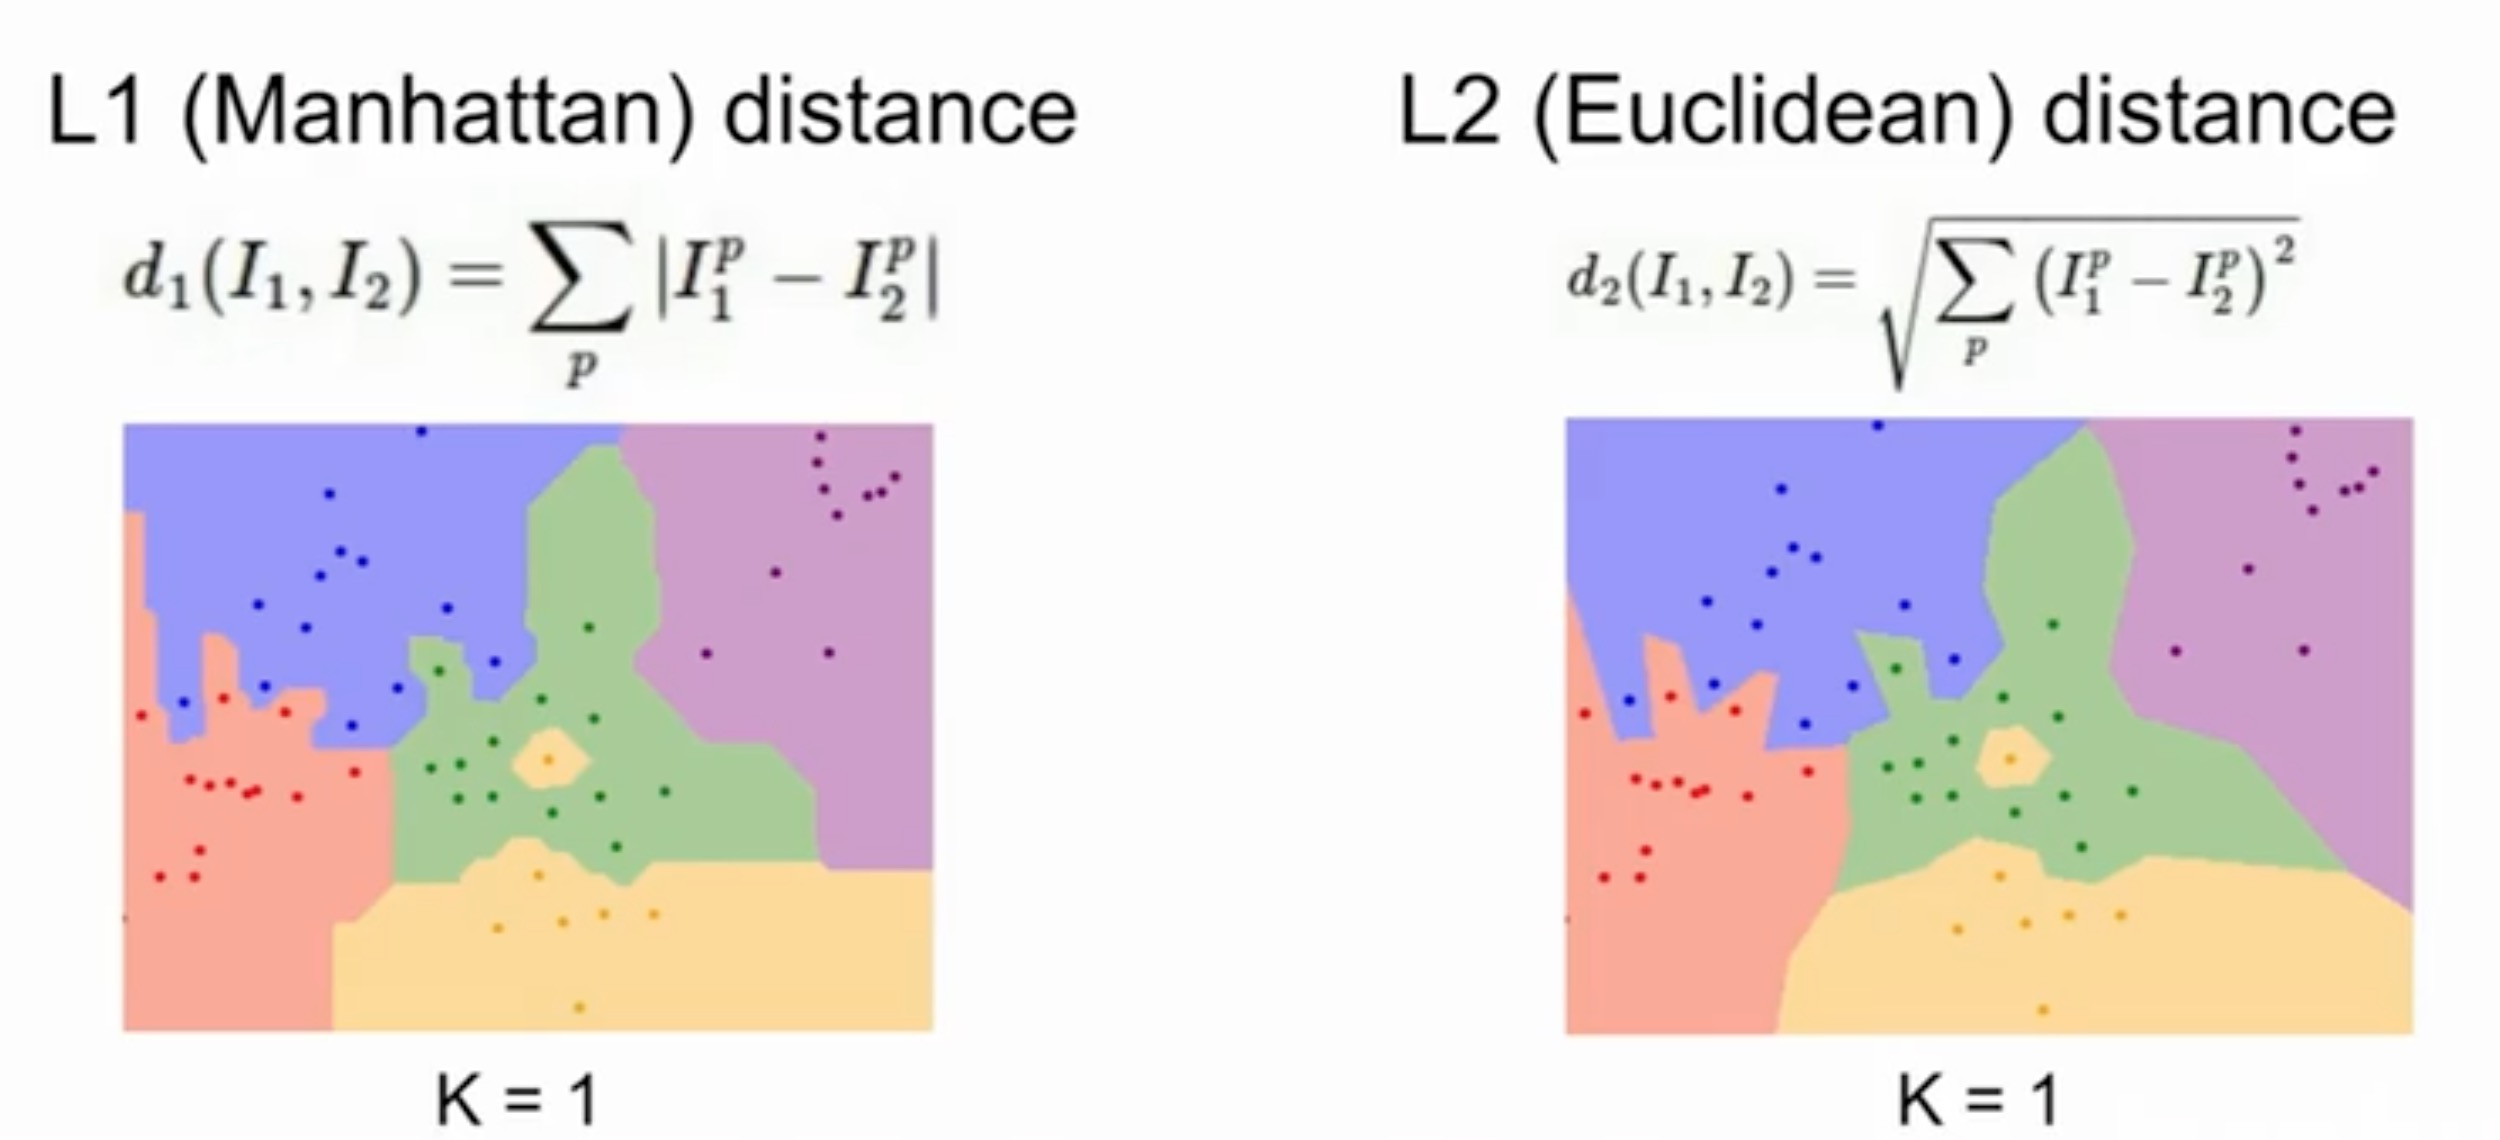
\includegraphics[width=0.7\linewidth]{figs/chapter1/nn l1 l2.jpg}
\end{figure}

\paragraph{训练、验证与测试集}
为了找寻最好的超参数，我们需要将数据集分为 $3$ 类：训练集、验证集、测试集. 选取一组超参数后，我们在训练集上训练模型，在验证集上测试该模型的性能，调整超参数使得性能达到最佳，最后在测试集进行测试，并以测试集上的性能作为该模型的真正性能。

\paragraph{交叉验证}

在数据集不是很多的时候，我们可以选择 $k$ 折交叉验证的方式代替上述方式。我们分出一部分测试集后，把剩下的数据集分成 $k$ 份（fold），循环地将每一份都视为验证集、其他份视为训练集进行 $k$ 次训练，以 $k$ 个训练性能的平均视为当前超参数下的训练性能，然后对超参数进行调整使得性能达到最佳，同样最后以在测试集上的性能作为真正性能。

\begin{figure}[H]
    \centering
    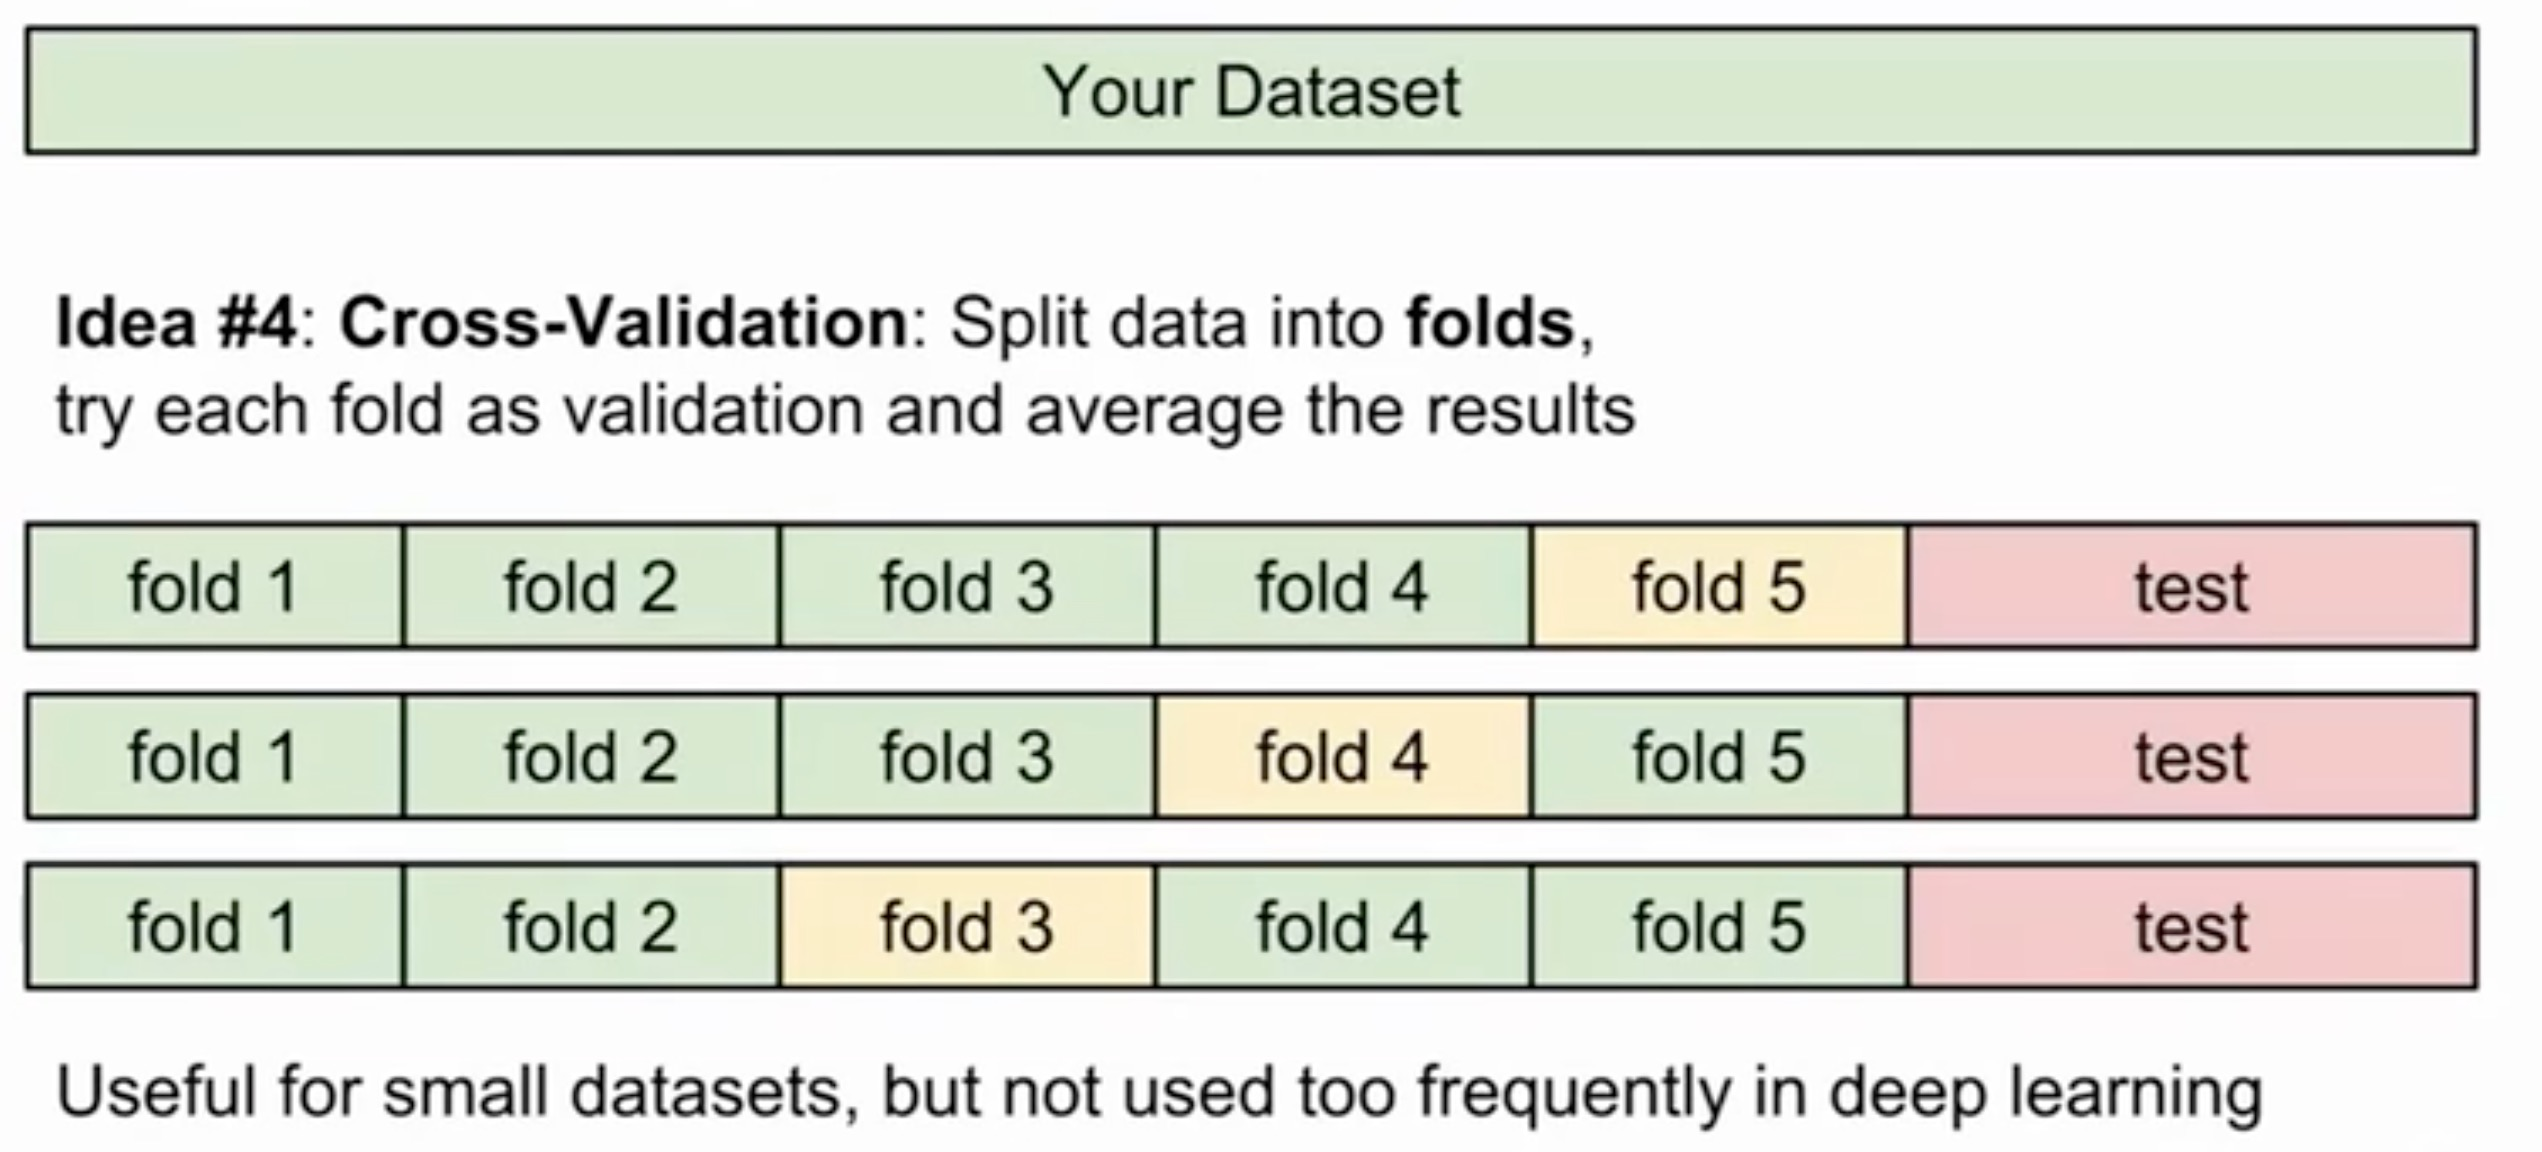
\includegraphics[width=0.6\linewidth]{figs/chapter1/cross validation.jpg}
\end{figure}


\paragraph{KNN 不被使用}

KNN 算法非常简单，但是问题也非常突出：

\begin{enumerate}
    \item 它基本没有训练过程，仅仅是把数据集记录下来，而在预测时需要遍历整个数据集，非常耗时（如果使用 KD-Tree 实现，随机数据下复杂度是 $\log$ 的，要好一些，但是仍然不满意）；这与我们需要的正好相反——我们愿意花费较多的时间对模型进行训练，但一旦训练好了，在对新数据预测时要很快地出结果。
    \item 不同的图像之间可以有相同的距离，这种度量方式对图像而言不太好。
    \item 当向量维度很高时，我们的数据点在高维空间中的分布是稀疏的，所以所谓的“最近点”可能其实并没有多么相似。
\end{enumerate}
